\section{Regulacja czasooptymalna}
\label{sec:toc}

W niniejszym podrozdziale przedstawiona została koncepcja regulacji czasooptymalnej. Zostały podane założenia zagadnienia, twierdzenia, na których podstawie można wyliczyć rozwiązanie oraz jego proponowana forma analityczna.

Zaznacza się, że mimo iż podane niżej definicje i założenia są wzięte z ogólnych zagadnień optymalizacji dynamicznej, to w podanym brzmieniu stosują się tylko do zagadnienia wyznaczania sterowania czasooptymalnego.

%-------------------------------------------------
\subsection{Ogólna definicja zagadnienia}
\label{sub:toc-def}

%-------------------
\subsubsection{Założenia wstępne}
\label{sub:toc-def-intro}
Dany jest układ opisany stacjonarnym, zwyczajnym równaniem różniczkowym (pokazanym jako równanie \ref{eq:general_system}), w którym:

\begin{equation}\label{eq:general_system}
    \frac{\partial x(t)}{\partial t} = f(x(t), u(t)), ~ 0 \leq t \leq T
\end{equation}

\begin{itemize}
    \item wektor zmiennych stanu w chwili $t$ - $x(t)$ spełnia następujące założenia:
    \begin{itemize}
        \item $\forall_{t \geq 0}:~ x(t) \in \mathbb{R}^{n}$ - ma $n$ składowych, a więc rozważany system ma $n$ równań różniczkowych zwyczajnych,
        \item $x(0) = x_{0} \in \mathbb{R}^{n}$ - spełnia warunek początkowy $x_{0}$;
    \end{itemize}
    \item wektor sterowań w chwili $t$ - $u(t)$:
    \begin{itemize}
        \item $\forall_{t \geq 0}:~ u(t) \in D \subset \mathbb{R}^{m}$ - ma $m$ składowych zawierającym się w zbiorze $D$ ograniczającym wartości sterowań,
        \item $u(0) = u_{0}$ - spełnia warunek początkowy $u_{0}$,
        \item funkcja $u$ jest przedziałami ciągła na przedziale $[0, T]$ (dokładny opis w \cite{Korytowski2015}), czyli:
        \begin{itemize}
            \item ma co najwyżej skończoną liczbę punktów nieciągłości,
            \item w każdym z nich ma skończoną granicę lewostronną,
            \item jest prawostronnie ciągła,
            \item w lewym końcu przedziału jest lewostronnie ciągła;
        \end{itemize}
    \end{itemize}
    \item funkcja $f: \mathbb{R}^{n} \times \mathbb{R}^{m} \longmapsto \mathbb{R}^{n}$:
    \begin{itemize}
        \item $f \in C^{1}$ - jest ciągła i różniczkowalna ze względu na pierwszy argument,
        \item $\frac{\partial f(t)}{\partial x} \in C^{0}$ - jej pochodna ze względu na pierwszy argument jest ciągła.
    \end{itemize}
\end{itemize}

Rozwiązaniem takiego równania jest oczywiście funkcja $x: [0, T) \longmapsto \mathbb{R}^{n}$ nazywana \emph{trajektorią układu}. 

Trajektoria będąca rozwiązaniem zagadnienia minimalnoczasowego musi spełniać następujący warunek końcowy (nazywany również stanem docelowym):
\begin{equation}\label{eq:final_term}
    x(T) = x_{f} \in \mathbb{R}^{n}
\end{equation}

Ów czas $T$, po którym przy danym sterowaniu stan systemu osiągnie warunek końcowy, będzie wskaźnikiem jakości: 
\begin{equation}\label{eq:quality}
    Q(u(t)) = q(x_{f}) = T
\end{equation}

Na tej podstawie można określić \emph{sterowanie optymalne} $\hat{u}(t)$, które spełnia wszystkie wspominane przy opisie równania \ref{eq:general_system} warunki oraz zależność \ref{eq:optimal_quality}. Trajektoria układu wygenerowana przez zastosowanie sterowania optymalnego nazwana jest \emph{trajektorią optymalną} i opisana symbolem $\hat{x}(t)$.
\begin{equation}\label{eq:optimal_quality}
    \forall_{u(t)}:~ Q(u(t)) \leq Q(\hat{u}(t))
\end{equation}

W opisie zagadnienia czasooptymalnego potrzebne są jeszcze dwa pojęcia.
Pierwsze to \emph{funkcja sprzężona} $\psi: [0, T] \longmapsto \mathbb{R}^{n}$ będąca rozwiązaniem tzw. równania sprzężonego \ref{eq:costate-def}.
\begin{equation}\label{eq:costate-def}
\frac{\partial \psi(t)}{\partial t} = - \frac{\partial f(x(t), u(t)}{\partial x}
\end{equation}

Tak, jak w przypadku trajektorii optymalnej układu, trajektoria $\psi(t)$ wyznaczona w układzie, w którym zastosowane zostało sterowanie optymalne $\hat{u}(t)$, nosi nazwę \emph{trajektorii sprzężonej optymalnej} i oznaczona jest symbolem $\hat{\psi}(t)$.

Ostatnim pojęciem potrzebnym w niniejszym zagadnieniu jest \emph{hamiltonian}, zwany również \emph{funkcją Hamiltona}, czyli funkcja $H: \mathbb{R}^{n} \times \mathbb{R}^{n} \times \mathbb{R}^{m} \longmapsto \mathbb{R}$ który dla trajektorii układu $x(t)$ wygenerowanej przy pomocy sterowania $u(t)$ i odpowiadającej im trajektorii sprzężonej $\psi(t)$ zdefiniowany jest zależnością \ref{eq:hamiltonian-def}.

\begin{equation}\label{eq:hamiltonian-def}
H(\psi(t), x(t), u(t)) = \psi(t) \circ f(x(t), u(t)) = \psi(t)^{T} \cdot f(x(t), u(t))
\end{equation}

%-------------------
\subsubsection{Zasada maksimum Pontriagina}
\label{sub:toc-def-pontriagin}

Aby jednoznacznie opisać, a następnie wyznaczyć sterowanie czasooptymalne, potrzebne jest przytoczenie zasadniczego twierdzenia w optymalizacji dynamicznej. Jest ono znane pod nazwą \emph{zasada maksimum Pontriagina}. Zostało opracowane w 1956 r. przez rosyjskiego matematyka Lwa Pontriagina. Twierdzenie podaje się w brzmieniu z \cite{Korytowski2015}.

\begin{pontriagin-max}\label{the:pontryagin}
    Zakładając układ opisany równaniem \ref{eq:general_system} z warunkiem końcowym \ref{eq:final_term} i wskaźnikiem jakości \ref{eq:quality} oraz równanie sprzężone \ref{eq:costate-def}:
    jeśli dla trajektorii układu $\hat{x}(t)$ wygenerowanej przy pomocy sterowania $\hat{u}(t)$ i odpowiadającej im trajektorii sprzężonej $\hat{\psi}(t)$ zachodzi:
    \begin{equation}\label{eq:pontriagin}
    \forall_{u(t) \in D}~ \forall_{t \in [0, T]}:~ H(\hat{\psi}(t), \hat{x}(t), \hat{u}(t)) ~ \geq ~ H(\hat{\psi}(t), \hat{x}(t), u(t))
    \end{equation}
    to sterowanie $\hat{u}(t)$ jest sterowaniem optymalnym.
\end{pontriagin-max}

Dowód zasady maksimum nie został uwzględniony w tej pracy. Można go znaleźć w \cite{Korytowski2015} oraz w \cite{Evans}.

Powyższe twierdzenie należy obwarować dodatkowymi warunkami koniecznymi optymalności. Niech funkcja $g: \mathbb{R}^{2n} \longmapsto \mathbb{R}^{l}$ opisuje zestaw ograniczeń nierównościowych, a funkcja $h: \mathbb{R}^{2n} \longmapsto \mathbb{R}^{k}$ - ograniczeń równościowych. Obie dane są wzorem \ref{eq:pontryagin-constraints}. Dodatkowo zakłada się, że $g, h \in C^{1}$.
\begin{equation}\label{eq:pontryagin-constraints}
    \begin{array}{lr}
    g(x_{0}, x_{f}) \leq 0 \\
    h(x_{0}, x_{f}) = 0
    \end{array}
\end{equation}

Ponadto, zakłada się, że istnieją $\lambda \in \mathbb{R}$, $\mu \in \mathbb{R}^{l}$ oraz $\rho \in \mathbb{R}^{k}$, które wraz z uprzednio zdefiniowanymi wielkościami i funkcjami spełniają następujące \emph{warunki konieczne optymalności}:
\begin{itemize}
    \item warunek nieujemności:
    \begin{equation}\label{eq:pontryagin-noneg}
    \lambda \geq 0 \land \|\mu\| \geq 0
    \end{equation}
    \item warunek nietrywialności:
    \begin{equation}\label{eq:pontryagin-notriv}
    \lambda + \|\mu\| + \|\rho\| > 0
    \end{equation}
    \item warunek komplementarności:
    \begin{equation}\label{eq:pontryagin-comp}
    \mu \circ g(x_{0}, x_{f}) = 0
    \end{equation}
    \item warunki transwersalności:
    \begin{equation}\label{eq:pontryagin-trans}
    \begin{array}{lr}
        \hat{\psi}(0) = \frac{\partial (\mu \circ g + \rho \circ h)}{\partial x_{0}}\\[8pt]
        \hat{\psi}(T) = - \frac{\partial (\mu \circ g + \rho \circ h)}{\partial x_{f}}\\[8pt]
        \forall_{t \in [0, T]}:~ H(\psi(t), x(t), u(t)) = \frac{\partial (\lambda T + \mu \circ g + \rho \circ h)}{\partial T} = \lambda
    \end{array}
    \end{equation}
    \item równanie sprzężone dane wzorem \ref{eq:costate-def},
    \item warunek maksimum hamiltonianu dany nierównością \ref{eq:pontriagin}.
\end{itemize}


%-------------------------------------------------
\subsection{Nieliniowość układu a sterowanie czasooptymalne}
\label{sub:toc-nonlnr}

Poszukiwanie sterowania czasooptymalnego w systemach nieliniowych jest skomplikowane, przede wszystkim ze względu na trudność rozwiązania analitycznego nieliniowych (lub nawet niestacjonarnych) równań różniczkowych. Układ zbiorników omawiany w niniejszej pracy jest również takimi opisany: zarówno równania dynamiki układu \ref{eq:model}, jak i równania sprzężone \ref{eq:model-costate} są nieliniowe.

Aby uprościć analizę problemu oraz fizyczne zastosowanie wyznaczonego sterowania, zakłada się, że poszukiwane jego postaci będą klasy ,,bang - bang''. To znaczy, że będą przyjmowały tylko wartości z brzegów jednowymiarowego zbioru dopuszczalnego $D \in \mathbb{R} \land D = [0, u_{max}] \Rightarrow \forall_{t \in [0, T]}:~ u(t) \in [0, u_{max}]$.

\begin{equation}\label{eq:nonlin-bang-bang}
    \frac{\partial x}{\partial t} = f(x(t)) + \sum_{i=1}^{m} g_{i}(x(t)) \cdot u_{i}(t)
\end{equation}

Można przyjąć takie założenie, ze względu na to, iż dla układów, których równania mają postać opisaną równaniem \ref{eq:nonlin-bang-bang}, funkcja przełączająca ma postać: $\phi(t) = \hat{\psi}(t) \circ g(\hat{x}(t))$. Opisano taką sytuację w \cite{YiMa2008} oraz w rozdziale 7.10 \cite{AthansOptCtrl}. Taka sytuacja zachodzi w omawianym układzie, gdzie $m = 1$.
Funkcja przełączająca opisuje momenty, w których sterowanie zmienia swoją wartość z jednego krańca zbioru $D$ na drugi. W przypadku rozważanego układu zbiorników sterowanie optymalne będzie dane wzorem \ref{eq:model-opt-ctrl}.

\begin{equation}\label{eq:model-opt-ctrl}
\begin{array}{lr}
    \hat{u}(t) = \frac{sgn(\phi(t)) + sgn(\phi(t))^{2}}{2} \cdot u_{max} ~ \land ~ \phi(t) = \frac{\hat{\psi}_{1}(t)}{aw} \Rightarrow \\
    \hat{u}(t) = \frac{sgn(\hat{\psi}_{1}(t) + sgn(\hat{\psi}_{1}(t))^{2}}{2} \cdot u_{max}
\end{array}
\end{equation}

Dodatkowo, jak wspomniano w podrozdziale \ref{sec:model}, układ otwarty jest stabilny, a ograniczone sterowanie nie może tego zmienić.

Podobne założenia są częstą praktyką w analizie stabilnych systemów nieliniowych ze względu na prostotę fizycznej aplikacji sterowania ,,bang - bang''. Przykłady znajdują się m.in. w \cite{VakKek82}, \cite{BalSom83} oraz \cite{Itik2016}.

%-------------------------------------------------
\subsection{Analityczne metody wyznaczania sterowania czasooptymalnego}
\label{sub:toc-ctrl}

Analityczne rozwiązania poszukiwania sterowania czasooptymalnego zwykle opierają się bezpośrednio na przytoczonej powyżej zasadzie maksimum i warunkach koniecznych optymalności. W niniejszym podrozdziale zostanie pokrótce przedstawiona droga mogąca zmierzać do wyznaczenia analitycznego czasooptymalnego sterowania w rozważanym układzie zbiorników. W niniejszej pracy całe rozwiązanie analityczne nie zostało przeprowadzone ze względu na fakt, iż równania sprzężone są niestacjonarne, a więc ich rozwiązanie analityczne byłoby bardzo trudne lub wręcz niemożliwe. Poniżej przedstawiono tylko kroki, które mogłyby prowadzić do takiego rozwiązania, gdyby dało się rozwiązać analitycznie równania sprzężone.

Pierwszym krokiem ku wyliczeniu analitycznego rozwiązania jest wyznaczenie równań sprzężonych za pomocą wzoru \ref{eq:costate-def}. Przyjmując współczynniki $\alpha_{i} = \frac{1}{2} \forall_{i \in \{1, 2, 3\}}$ w modelu matematycznym zestawu zbiorników danym równaniem \ref{eq:model}, można wyznaczyć równania sprzężone rozważanego układu. Są one dane wzorem \ref{eq:model-costate}. Pominięto w nim zależności wszystkich funkcji $\psi$ oraz $h$ od czasu, aby uprościć zapis.

\begin{equation}\label{eq:model-costate}
	\left \{
	\begin{array}{lr}
		\frac{\partial \psi_{1}}{\partial t} =  \psi_{1}\frac{C_{1}}{2aw\sqrt{h_{1}}} - \psi_{2}\frac{C_{1}}{2\sqrt{h_{1}}(cw + \frac{h_{2}}{h_{max}}bw)} \\[20pt]
		\frac{\partial \psi_{2}}{\partial t} = - \psi_{2}\frac{1}{cw + \frac{h_{2}}{h_{max}}bw}(\frac{b(C_{1}\sqrt{h_{1}} - C_{2}\sqrt{h_{2}})}{ch_{max} + bh_{2}} - \frac{C_{2}}{2\sqrt{h_{2}}}) - \psi_{3}\frac{1}{w\sqrt{h_{3}(2R - h_{3})}} \\[20pt]
		\frac{\partial \psi_{3}}{\partial t} = \psi_{3}\frac{-C_{3}(3R - 2h_{3})}{wh_{3}(2R - h_{3})^{\frac{3}{2}}}
	\end{array}
	\right.
\end{equation}

Następnie trzeba by przedefiniować ograniczenia równościowe (dane wzorem \ref{eq:model-eq-const}) i nierównościowe (\ref{eq:model-noneq-const}) tak, aby spełniały założenia funkcji $g$ i $h$ opisane zależnościami \ref{eq:pontryagin-constraints}.
Dodatkowo należy dopisać od ograniczeń równościowych to wynikające z faktu poszukiwania sterowania czasooptymalnego, czyli \ref{eq:final_term}, które w tym przypadku będzie miało postać opisaną przez \ref{eq:model-final-term}, gdzie $h_{1f}$, $h_{2f}$ i $h_{3f}$ są dane.

\begin{equation}\label{eq:model-final-term}
\begin{array}{lr}
    h_{1}(T) = h_{1f}\\
    h_{2}(T) = h_{2f}\\
    h_{3}(T) = h_{3f}
\end{array}
\end{equation}

Korzystając z warunków komplementarności (\ref{eq:pontryagin-comp}) oraz nieujemności (\ref{eq:pontryagin-noneg}), powinno się wyznaczyć składowe wektora $\mu$ oraz założyć pewną postać wektora $\rho$ (bazując takie założenie na \ref{eq:pontryagin-notriv}).

Na podstawie tych danych należałoby wyznaczyć warunki początkowy i końcowy danym wzorem \ref{eq:pontryagin-trans} dla powyższych równań sprzężonych, co pozwoliłoby wyznaczyć analityczne wzory opisujące wszystkie składowe trajektorii sprzężonych systemu.

Na koniec, korzystając z zależności \ref{eq:model-opt-ctrl}, można by wyznaczyć analityczny wzór sterowania optymalnego.


%-------------------------------------------------
\subsection{Numeryczne metody wyznaczania sterowania czasooptymalnego}
\label{sub:toc-num}

W niniejszej sekcji zostały przekrojowo zaprezentowane numeryczne metody poszukiwania sterowania czasooptymalnego dla układów nieliniowych.
Nie jest jej celem przedstawienie dokładnego działania wszystkich istniejących algorytmów, lecz dokonanie klasyfikacji i naświetlenie interesujących metod oraz odesłanie do odpowiedniej literatury przedmiotu.

Ogólna definicja problemu optymalizacji rozwiązywanego przez takie metody została dana w sekcji \ref{sub:toc-def}. Tutaj należy ją uzupełnić o ogólną postać funkcjonału $Q$ będącego wskaźnikiem jakości w rozpatrywanym zadaniu. Jest ona dana równaniem \ref{eq:num-oc-quality} (za: \cite{Rao2010}) i składa się z:
\begin{itemize}
    \item wyrażenia podcałkowego $L$ zależącego od:
    \begin{itemize}
        \item czasu,
        \item stanu $x(t)$,
        \item sterowania $u(t)$,
        \item parametrów statycznych układu $p$,
        \item czasu końcowego $T$;
    \end{itemize}
    \item wyrażenia $M$ zależącego od:
    \begin{itemize}
        \item czasu początkowego optymalizacji $t_{0}$,
        \item stanu początkowego $x(t_{0})$,
        \item stanu końcowego $x(T)$,
        \item parametrów statycznych układu $p$,
        \item czasu końcowego $T$.
    \end{itemize}
\end{itemize}

\begin{equation}\label{eq:num-oc-quality}
Q[x(\cdot), u(\cdot), p, t_{0}, T] = \int_{t_{0}}^{T}L(\tau, x(\tau), u(\tau), p, T)d\tau + M(t_{0}, x(t_{0}), x(T), p, T)
\end{equation}

Gdy we wskaźniku jakości występuje tylko człon podcałkowy, to mówi się, że jest postaci Lagrange'a. Jeśli ma tylko drugi człon, nazywa się go postacią Mayera. Sytuację, w której występują oba, określa się mianem postaci Boltza (za: \cite{Rao2010}). Oczywiście, podział między członami jest umowny i można ten sam funkcjonał zapisać zarówno w postaci Lagrange'a, jak i Mayera. Przykładem jest rozpatrywany w niniejszej pracy wskaźnik jakości dany postacią Mayera we wzorze \ref{eq:quality}. Równie dobrze można by go zapisać w postaci Lagrange'a: $Q = \int_{0}^{T} 1 ~d\tau$.

Podstawowy podział metod obliczeniowych to metody \emph{pośrednie} oraz \emph{bezpośrednie}, choć ich rozróżnienie nie jest ścisłe i istnieją metody łączące cechy obu tych klas (za: \cite{Betts98}).

Pierwsze z nich polegają na dyskretyzacji sterowania (czasem również stanu), aby móc przybliżyć wyjściowy problem optymalizacji dynamicznej zadaniem optymalizacji statycznej: programowania nieliniowego (ang. \emph{NLP - Non-Linear Programming}). To przybliżenie jest zwykle aproksymacją sterowań (oraz stanów w tych metodach, które z nich korzystają) w konkretnych przedziałach czasu wielomianami. Dzięki temu zastępuje się nieskończenie wymiarowy problem optymalizacji takim o skończonym wymiarze.
Metody bezpośrednie dzieli się na:
\begin{itemize}
    \item metody \emph{sekwencyjne}, które używają wysokiej klasy oprogramowania do całkowania sterowania, aproksymowanego wielomianami i traktują wyliczone na jego podstawie trajektorie jako dokładne,
    \item metody \emph{równoczesne}, które korzystają z parametrycznej aproksymacji trajektorii układu uzyskanej w wyniku kolokacji.
\end{itemize}

Ta klasa metod jest bardziej uniwersalna i mniej wrażliwa na błędy, ale stosunkowo wolniej zbieżna i przez to mniej dokładna (za: \cite{Korytowski2015}).
Przykładowe metody bezpośrednie przedstawione są poniżej:
\begin{itemize}
    \item optymalizacja czasów przełączeń (do zastosowania tylko w przypadku sterowania o postaci ,,bang-bang''),
    \item parametryzacja sterowania (np. aproksymacja funkcją schodkową),
    \item bezpośrednie metody kolokacyjne,
    \item metody strzałów bezpośrednich.
\end{itemize}

Metody pośrednie wykorzystują warunki konieczne optymalności oryginalnego zadania i sprowadzają je do problemu granicznego lub dwugranicznego, który jest dany układem równań bazującym na zasadzie maksimum Pontriagina. Rozwiązanie takiego układu równań skutkuje wyznaczeniem trajektorii układu będących potencjalnie rozwiązaniem problemu. Każdą z nich bada się, jakeigo rodzaju ekstremem jest: minimum, maksimum lub punktem siodłowym, a następnie wybiera się taką, której koszt jest najmniejszy. Metody pośrednie wymagają dobrze dobranej trajektorii początkowej układu, która zawiera informacje na temat struktury sterowania (za: \cite{Korytowski2015}). Jest to wada tego rodzaju metod - wymagają większego nakładu pracy analitycznej przed rozpoczęciem obliczeń, aby wyznaczyć odpowiedni punkt startowy dla algorytmu. Zaletą za to jest dużo szybsza zbieżność w otoczeniu rozwiązania (za: \cite{Korytowski2015}). Przykładowe metody pośrednie to:
\begin{itemize}
    \item pośrednia metoda strzałów,
    \item pośrednia metoda strzałów wielokrotnych,
    \item pośrednie metody kolokacyjne.
\end{itemize}

Rys. \ref{fig:num-methods} przedstawia operacje matematyczne wykorzystywane przez oba rodzaje metod rozwiązywania problemów optymalizacji dynamicznej. Dokładniejszy opis metod wykonujących te operacje znajduje się w \cite{Rao2010}. W niniejszej pracy również zawarto ich opis w sekcji \ref{sub:opt-alg}.

\begin{figure}[htp]
    \centering
    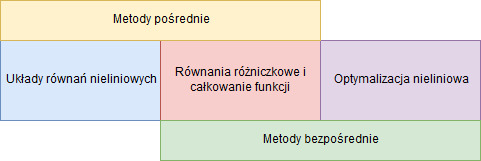
\includegraphics[scale=0.8]{Grafika/num-methods}
    \caption{Trzy główne komponenty wyznaczania sterowania optymalnego i klasy metod, które z nich korzystają. Źródło: \cite{Rao2010}. Tłumaczenie: własne.}
    \label{fig:num-methods}
\end{figure}
